\section{Method}
\label{sec:method}

\subsection{Problem formulation}
Given an ultrasound region-of-interest (ROI) image $x$, the goal is to predict the lesion label $y \in \{0,1\}$ for benign--malignant classification, where $0$ denotes benign and $1$ denotes malignant. The model outputs a two-dimensional logit vector $z=f_{\theta}(x)$, and the malignant posterior is computed as
\begin{equation}
    p(y=1\mid x) = \frac{\exp(z_1)}{\exp(z_0) + \exp(z_1)}.
\end{equation}
The main paper uses the same binary formulation across TN5000, BUSI, and AUL, so that the proposed architecture can be evaluated under a unified lesion-classification setting.

\subsection{ROI-based input construction}
Figure~\ref{fig:roi_preprocessing} summarizes the input construction. The lesion annotation defines the initial bounding box. The box is expanded around the lesion center, converted to a square crop, clipped to the image boundary, and resized to the model input size. This procedure keeps the lesion centered while retaining a controlled amount of surrounding tissue context. The main classification protocol therefore uses annotation-derived ROI crops; a separate closed-loop experiment in Section~\ref{sec:experimental_setup} evaluates detector-predicted ROI crops as an auxiliary inference-time front end.

\begin{figure}[t]
    \centering
    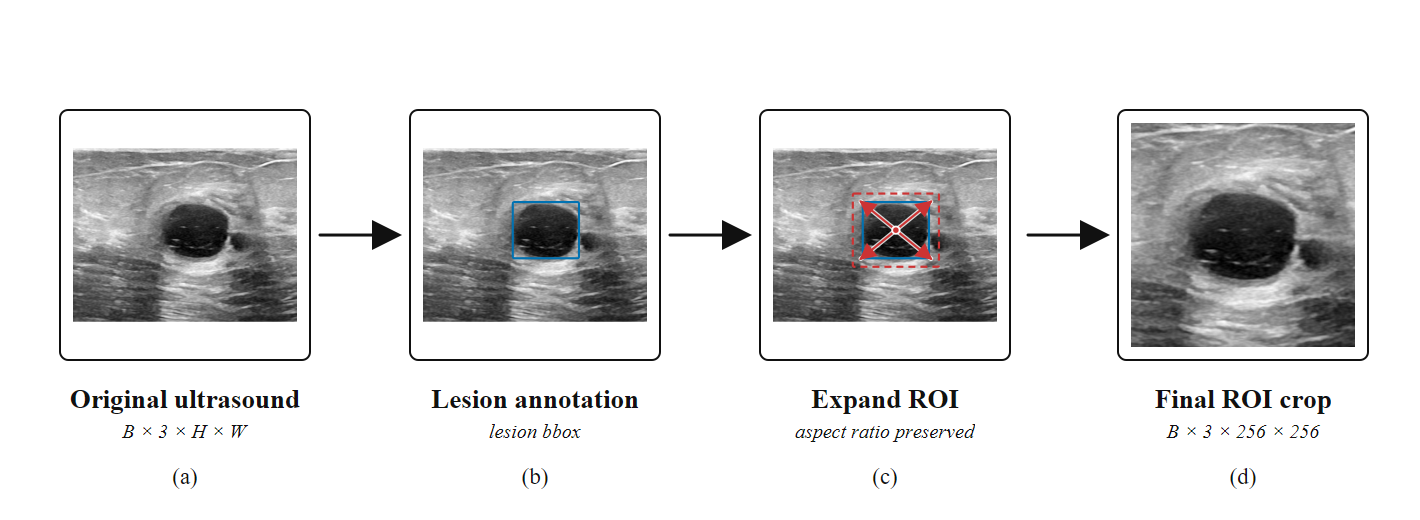
\includegraphics[width=0.92\textwidth]{fig_roi_preprocessing.png}
    \caption{ROI-based input construction. The lesion annotation defines the initial bounding box; an expanded square crop centered on the lesion is extracted and resized to the model input size.}
    \label{fig:roi_preprocessing}
\end{figure}

\subsection{Overall architecture}
Figure~\ref{fig:architecture} illustrates UL-TransXNet, the architecture used in the main experiments. A $256 \times 256$ ROI crop is processed by a lightweight four-stage hierarchical backbone. The backbone follows the tiny TransXNet family configuration with stage depths $[4,4,15,4]$, embedding dimensions $[48,96,224,448]$, head numbers $[1,2,4,8]$, and spatial-reduction ratios $[8,4,2,1]$. Each block keeps the central TransXNet idea of local--global token mixing: local convolutional dynamics preserve fine lesion structure, while the global branch models broader contextual relationships.

The backbone is used as a feature extractor and outputs a 1000-D representation. A lightweight task head maps this representation to the final binary prediction through a two-layer multilayer perceptron, $1000 \rightarrow 512 \rightarrow 2$, with GELU activation and dropout between the two linear layers. This keeps the classifier head simple and makes the backbone design the main source of representation capacity.

\begin{figure}[t]
    \centering
    
\includegraphics[width=0.96\textwidth]{fig_architecture.png}
    \caption{Overview of UL-TransXNet. The ROI crop is resized to $256 \times 256$ and processed by hierarchical patch/stem embedding, four TransXNet stages, global pooling, and a lightweight MLP head. The lower panel abstracts the representative block used to describe local/global token mixing, residual fusion, and MS-FFN refinement.}
    \label{fig:architecture}
\end{figure}

\subsection{Progressive TransXNet family refinements}
Rather than treating the final model as a one-shot design, we organize the architecture as a progressive refinement of the TransXNet baseline~\cite{transxnet}. The baseline, denoted \texttt{TransXNet}, already combines dynamic local convolution and global attention in a compact hierarchical backbone. The ultrasound setting motivates additional refinements because lesion boundaries can be weak, discriminative textures can be local, and useful context can appear at different spatial scales.

The first refinement, \texttt{TransXNet-G}, enables multi-scale coordinate attention (MCA), inspired by coordinate attention for lightweight networks~\cite{hou2021coordinate}, in selected global-branch locations. The intent is to improve spatially aware feature selection without a large complexity increase. The second refinement, \texttt{TransXNet-GG}, adds multiway dynamic dense connections (MUDD) in deeper stages to encourage short-range feature reuse. The \texttt{TransXNet-GGG} variant introduces differential attention in the later global branch. We denote the deployed main model as \textbf{UL-TransXNet}; in the ablation notation, it corresponds to the \texttt{TransXNet-GGG-MCA} configuration. This naming keeps the final model separate from the internal G/GG/GGG identifiers used for ablation. UL-TransXNet is used as the main cross-dataset model because the selection criterion is average behavior across TN5000, BUSI, and AUL rather than the TN5000-only optimum. The TN5000 ablations also show that the intermediate \texttt{TransXNet-GG} variant can be the strongest single TN5000 structure. This is an important part of the evidence rather than a contradiction: the refinements improve different operating characteristics, and MCA should be interpreted as a robustness-oriented module rather than as a guaranteed AUC-improving switch.

\subsection{Key modules}
\paragraph{Multi-scale coordinate attention (MCA).}
When enabled, MCA operates on the global branch after channel splitting. It partitions channels into multiple scale groups, pools each group at a different spatial scale, injects coordinate-aware responses, and generates attention weights for spatially selective feature recalibration. In ultrasound images, lesions may differ through both coarse shape and fine echo patterns; MCA is intended to retain this scale diversity while keeping attention lightweight.

\paragraph{Multiway dynamic dense connection (MUDD).}
MUDD is inserted in deeper stages, where semantic features are richer but optimization can be harder. The block feature is divided into multiple channel paths, and a lightweight weight generator computes path-wise aggregation weights from the current activation. Previous block features from the same stage are dynamically fused through these paths. This gives the deeper stages a compact adaptive memory without turning the backbone into a heavy dense network.

\paragraph{Differential attention.}
The \texttt{GGG} variant replaces the standard global attention unit in selected later-stage locations with differential attention, within the general attention-based modeling framework introduced by Transformer architectures~\cite{vaswani2017attention}. Queries and keys are split into two halves, the second query half is normalized, and two attention maps are formed and subtracted with a learnable balancing coefficient. The goal is to sharpen relational contrast in the global branch, which is useful when benign and malignant lesions share broad ultrasound appearance statistics but differ in subtle internal organization.

These modules are introduced as a progressive design family, not as a full factorial decomposition. The ablation study therefore reports both structure-level variants and core-module variants to make the interpretation explicit.

\subsection{Complexity analysis}
Table~\ref{tab:complexity} reports the complexity of the comparison pool and the TransXNet family variants. The numbers are measured with the same binary-classification wrapper used by the training scripts, so they include both the backbone and the lightweight MLP head. All models use $256 \times 256$ ROI inputs except EfficientFormer-L1, which follows its $224 \times 224$ setting. UL-TransXNet is not the smallest model in the pool, but it remains substantially lighter than the strongest TN5000 baselines ConvNeXt-Tiny and Swin-T while preserving stronger cross-dataset behavior on BUSI and AUL.

\begin{table*}[t]
    \centering
    \small
    \caption{Model complexity of the comparison pool and TransXNet family variants. Parameters and MACs are measured for the full binary classifier, including the lightweight MLP head. MACs are reported for one forward pass at the listed input size.}
    \label{tab:complexity}
    \resizebox{\textwidth}{!}{%
    \begin{tabular}{llccc}
        \toprule
        Method & Role & Input & Params (M) & MACs (G) \\
        \midrule
        ResNet50 & Prior baseline & $256 \times 256$ & 24.56 & 5.40 \\
        DenseNet121 & Prior baseline & $256 \times 256$ & 7.48 & 3.70 \\
        EfficientNet-B0 & Prior baseline & $256 \times 256$ & 4.66 & 0.50 \\
        MobileNetV3-Large & Prior baseline & $256 \times 256$ & 4.86 & 0.28 \\
        Swin-T & Prior baseline & $256 \times 256$ & 27.91 & 7.11 \\
        ConvNeXt-Tiny & Prior baseline & $256 \times 256$ & 28.21 & 5.82 \\
        RepViT-M1.1 & Prior baseline & $256 \times 256$ & 8.04 & 1.80 \\
        EfficientFormer-L1 & Prior baseline & $224 \times 224$ & 11.62 & 1.31 \\
        TransXNet & Ours / ablation & $256 \times 256$ & 13.35 & 2.32 \\
        TransXNet-G & Ours / ablation & $256 \times 256$ & 13.42 & 2.34 \\
        TransXNet-GG & Ours / ablation & $256 \times 256$ & 14.15 & 2.38 \\
        TransXNet-GGG-noMCA & Ours / ablation & $256 \times 256$ & 14.29 & 2.34 \\
        \textbf{UL-TransXNet} & \textbf{Ours} & $256 \times 256$ & 14.37 & 2.36 \\
        \bottomrule
    \end{tabular}%
    }
\end{table*}

